\section{Forced-Sale Supply (FSS)}
\label{sec:fss}

\subsection{The flow instrument}

For each filer, implied quarterly flow separates client/leverage
money from market growth of the book:
\[
\mathrm{flow}_{m,t} \;=\; \frac{\mathrm{AUM}_{m,t}}{\mathrm{AUM}_{m,t-1}}
\;-\;\bigl(1 + r^{\text{book}}_{m,t}\bigr),
\]
with $r^{\text{book}}$ the frozen prior book marked on the price
panel. The instrument is validated against subsequent \emph{behavior},
not returns: managers with $\mathrm{flow} < -10\%$ sell 34.5\% of
held shares over the next quarter versus 23.1\% for managers with
positive flow ($t=+10.6$; the contrast against the strictest healthy
definition reaches $t=+20.9$). Completer books strengthened the
instrument (the campaign of Section~\ref{sec:campaign}), as a real
instrument should. Selling by distressed managers is approximately
pro-rata across the liquidity spectrum (liquidity-ordering
correlation $-0.02$): the folklore ``they sell the liquid names
first'' is not in this data.

\subsection{Threshold justification without selection}

The $-10\%$ cut was set a priori. Its justification is the
\emph{shape} of the mechanism, which involves no selection at all:
the sold-fraction delta versus healthy managers rises smoothly
through every threshold --- $+7.8$pp at $-5\%$, $+11.4$pp at
$-10\%$, $+13.9$pp at $-20\%$, each with $t$ between $+9.6$ and
$+11.4$ (Figure~\ref{fig:mechanism}). The default is a point on a
monotone curve, chosen where purity meets sample size (144 distressed
managers per quarter, versus 65 at $-20\%$).

\begin{figure}[t]
\centering
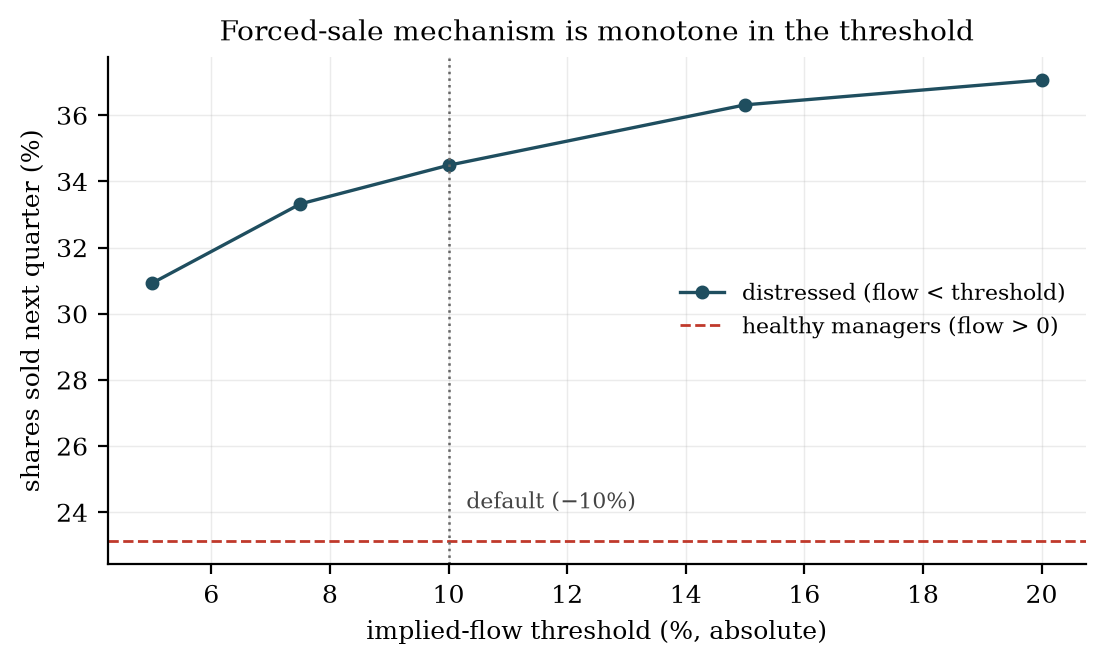
\includegraphics[width=.6\linewidth]{figs/f6_mechanism.png}
\caption{The forced-sale mechanism is monotone in the flow
threshold; the a-priori default is not a knife edge. No returns are
involved in this figure.}
\label{fig:mechanism}
\end{figure}

\subsection{From managers to stocks, and what the price says}

Stock-level supply aggregates each distressed manager's
prospective liquidation over average daily dollar volume:
$\mathrm{FSS}_{i,t}=\sum_{m \in \mathrm{dis}}
|\mathrm{flow}_{m,t}|\,\mathrm{AUM}_{m,t}\, w_{m,i,t} /
\mathrm{ADV}_{i,t}$. Pricing this basket honestly required a
benchmark audit that we report as a finding in its own right. Against
the universe \emph{mean}, the basket ``underperforms'' by
$3.8\%$/quarter --- but so does nearly everything: the cross-sectional
mean of quarterly stock returns sits $\sim$4\%/quarter above the
median through small-cap skewness, and early internal notes quoting a
$-4.5\%$/quarter cohort effect against the mean overstated the alpha.
Against the median the basket is flat. The tradable statement is the
index-hedged one: approximately flat 2013--2020 (Sharpe $-0.1$ to
$-0.5$ across all fifteen threshold$\times$basket configurations) and
\textbf{paying $+0.6$ to $+1.0$ Sharpe in 2021--2025} ($t$ up to
$+4.0$) at \emph{every} point of the grid. The grid moves as one
block: no configuration is special, none is fragile, and what the
surface identifies is a \emph{regime} --- the degrossing/rates era
--- rather than a hyperparameter.

The same surface furnishes a methodological result we consider as
valuable as the factor itself: the in-sample-to-out-of-sample rank
correlation across configurations is \emph{negative} ($-0.81$ for
the bootstrap 5th-percentile statistic). Under a regime flip, any
in-sample selector --- robust or naive --- is anti-informative. The
\citet{oliveira2025} machinery assumes a stationary utility
distribution; NCB's surface satisfies it (rank correlation $+0.53$)
and selection works there; FSS's does not, and the correct use of the
protocol is to refuse to select and report the regime
(Figure~\ref{fig:surfaces}, right). We apply our tools critically or
not at all.

\subsection{Prediction fails at every clock (Law 2)}

Three designs tried to move FSS from observation to anticipation, and
all failed their mechanism gates, which is why the production leg
reacts to filings rather than front-running them.
(i) \emph{Quarterly flow forecasting} in the \citet{coval2007}
expected-flow form (lagged flow + performance + convexity, expanding
coefficients): 13F-implied flow has no one-quarter-ahead
predictability (OOS rank correlation $-0.015$, $t=-1.21$);
predicted-distressed managers do not sell more than predicted-inflow
managers ($t=+0.69$, against $t=+20.9$ contemporaneous). The
literature forecasts \emph{reported} mutual-fund TNA flows;
13F-implied flow adds leverage, unreported assets, and frozen-book
error, which destroys the autocorrelation. (ii) \emph{Daily
synthetic stress}: retracted (Section~\ref{sec:campaign}).
(iii) \emph{Single-name crash cascades}: the middle link (salient
position crash $\to$ next-quarter redemption) does not clear its
bar ($t=-1.47$); redemptions respond to aggregate performance, which
the flow instrument already captures contemporaneously.
